\section{Angewandte Ansätze für die Erkennung von Design Patterns}

Bei der Erkennung von Design Patterns in Quellcode wurden verschiedene Verfahren entwickelt werden, die auf unterschiedlichen Methoden beruhen, um das gesetzte Ziel zu erreichen.
Yarahmadi et al.~führten in ihrer Arbeit eine Untersuchung über die Methoden, die angewandt worden, um Design Patterns in Quellcode zu erkennen, und kategorisierten diese~\cite[S. 5805]{yarahmadi2020design}.

\begin{figure}[h]
    \centering
    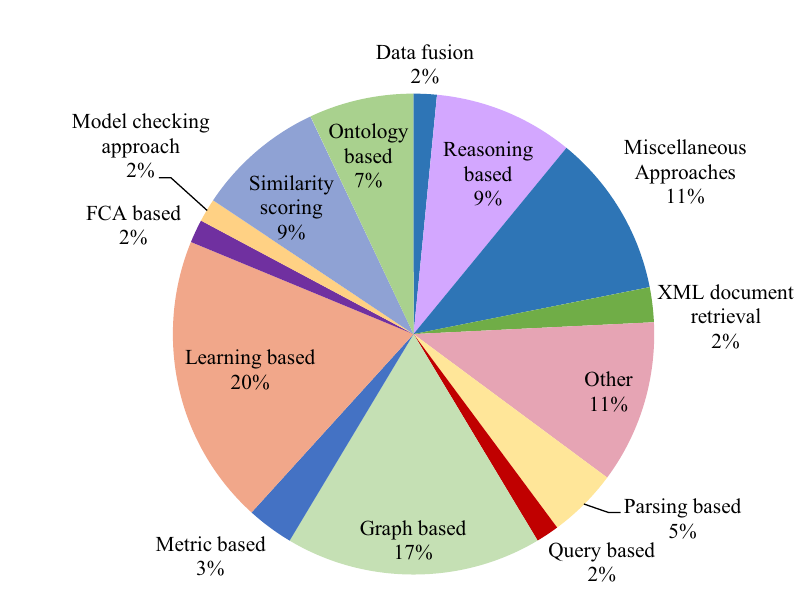
\includegraphics[scale=0.5]{figures/approches_distribution.png}
    \caption{Verteilung der Kategorien der Ansätze für die Erkennung von Design Patterns in Quellcode}
    \label{fig:approach_dist}
\end{figure}

Wie aus Figur~\ref{fig:approach_dist} zu entnehmen ist, wurden die entwickelten Prozesse von Yarahmadi et al. auf eine begrenzte Menge an Kategorien eingestuft.
In dieser Sektion der Arbeit werden die vier größten Kategorien aus Figur~\ref{fig:approach_dist} genauer erläutert und es werden exemplarisch Arbeiten diskutiert,
die in die jeweilige Kategorie zugeordnet werden können. 

\subsection{Graphen-basierende Ansätze}

Die Methodik der Reduktion stellt in der Berechenbarkeitstheorie einen Ansatz dar, um Lösungswege für neue unbekannte Probleme zu entwickeln. Dabei wird durch einen Algorithmus das unbekannte Problem in ein bereits gelöstes Problem, dessen Lösungsweg bereits vorhanden ist, umgewandelt.
In Graphen-basierenden Methoden für die Erkennung von Design Pattern in Quellcode wird diese angewendet, um Quellcode in Graphen zu transformieren und diese Graphen werden als Eingabe für diverse Graphenalgortihmen verwendet.

\pagebreak

Formell betrachtet ist ein Graph definiert als~\cite[S. 9]{Siu1998IntroductionTG}:
\begin{align*}
& \text{G} = \{V(G), E(G)\}
&\\
&\text{mit}
&\\
&G : \text{der zu betrachtende Graph}\\
&V (G): \text{Nicht leere Menge von Knoten in G}\\
&E (G): \text{Menge an ungeordneten Tupeln von distinkten Elementen von V (G)}
\end{align*}

Der Quellcode selbst ist als roher Text zu betrachten, welches verschiedene Entitäten wie Klassen, Objekte und Schnittstellen beinhaltet, und definiert, wie diese miteinander interagieren. Als Graph $G$ werden die Entitäten aus dem Quellcode als Knoten $V (G)$ und 
die Relationen und Interaktionen wie Vererbung oder Methodenaufrufe werden als Kanten $E (G)$ dargestellt.
Hierbei stellt Unified Modeling Language (UML) eine in der Software-Entwicklung verbreitete Modellierungssprache dar und definiert verschiedene Arten von Graphen dar, um Software und andere Systeme zu modellieren.
Die Diagramme aus der UML-Domäne werden in diesem Kontext als Graphen aufgefasst, da diese aus einer Menge aus Kanten und Konten bestehen und anhand der obigen Definition als Graphen interpretiert werden können.
Eine Diagrammart aus der Domäne, welches eingesetzt wird, um objektorientierte (OO) Software-Systeme zu modellieren, sind Klassendiagramme.
Klassendiagramme beschreiben, wie Klassen und deren Relation zueinander im Kontext des Paradigmas der OO-Programmierung aufgefasst werden.
Pradhan et al.\ nutzen Klassendiagramme als Eingabe für ihre entworfene Methode und generieren diese für das zu analysierende Software-System und Implementierung von Entwurfsmustern, die als Referenz genutzt werden~\cite[S. 2]{7346680}.
Diese werden als gerichtete Graphen erfasst, wobei die Klassen als Knoten und die Assoziation wie Vererbung zwischen diesen als Kanten darstellen. Zusätzlich werden die Kanten je nach Art der Assoziation unterschiedlich gewichtet~\cite[S. 2]{7346680}.
Im weiteren Verlauf werden mögliche Menge Kandidaten aus dem Graphen des Software-Systems als dessen Subgraphen durch die Eigenschaft der Graphenisomorphie extrahiert und anhand der normalisierten Kreuzrelation der Maß der Übereinstimmung bestimmt~\cite[S. 3]{7346680}.
Graphenisomorphie beschreibt, ob zwei Graphen die strukturell identisch sind, sodass jede Kante des einen Graphen einer Kante im anderen Graphen entspricht und umgekehrt~\cite[S. 10]{Siu1998IntroductionTG}. Die normalisierten Kreuzrelation ist ein Maß, dessen Wertebereich zwischen 0.0 und 1.0 definiert ist.
Je näher der Wert an 1.0, desto identischer sind die zwei Graphen. 
Zu der Evaluierung des Prozesses wurden vier Open Source Software-Systeme hergezogen, aus welchen fünf existierende Entwurfsmuster zu erkennen sind~\cite[S. 6]{7346680}. Dabei wurde von Pradhan et al. dokumentiert, ob ein Entwurfsmuster komplett oder partiell im Quellcode entdeckt wurde.
Nach eigener Auswertung von Pradhan et al. wurden die als Referenz genommen Implementierung der Design Patterns mehrfach komplett als auch partiell in der Codebasis der zu dem Test hergezogen Software-Systeme identifiziert~\cite[S. 6]{7346680}.

\pagebreak

In ihrer Arbeit verfolgen Dongjin et al. in ihrer vorgeschlagenen Methodik ebenfalls die Erkennung von Entwurfsmustern der strukturellen Kategorie in Quellcode durch den Einsatz von Graphen. In Kontext dieser werden wie im vorherigen Verfahren beschriebenen Klassendiagramme als gerichtete gewichtete Graphen eingesetzt.
Entitäten wie Klassen, Objekte oder Schnittstellen als Knoten und die Assoziation der Entitäten wie Vererbung als gerichtete gewichtete Kanten des repräsentiert~\cite[S. 582]{6649882}.
Zudem werden Referenzimplementierung der zu identifizierenden Entwurfsmuster in gewichtete Klassendiagramme transformiert und innerhalb dieser werden Submuster definiert, die in Summe das Entwurfsmuster repräsentieren~\cite[S. 580]{6649882}.

\begin{figure}[h]
    \centering
    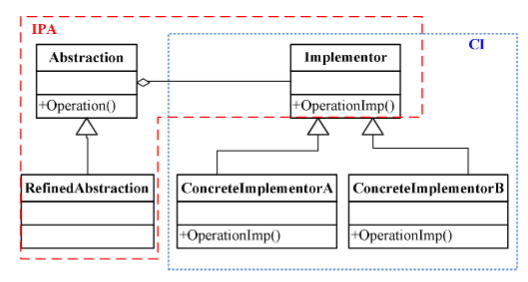
\includegraphics[scale=0.75]{figures/struture_bridge.png}
    \caption{Referenzklassendiagramm des Bridge Patterns mit Submustern}
    \label{fig:structure_bridge}
\end{figure}

Beispielhaft spiegelt die Abbildung \ref{fig:structure_bridge} von Dongjin et al. definierte Referenzklassendiagramm für das Bridge Pattern wider. Innerhalb dieses Klassendiagramms werden die Submuster \textbf{IPA} und \textbf{CI} festgelegt. Wie von der Abbildung \ref{fig:structure_bridge} zu entnehmen ist, bestehen die Submuster aus einzelnen Entitäten und deren Assoziationen.
Innerhalb der Klassendiagramme des Quellcodes, welches als Eingabe dient, wird nach solchen Submustern durch Einsatz von Graphenisomorphie gesucht~\cite[S. 584]{6649882}. Im weiteren Verlauf werden identifizierte relevante Submuster zu einer Kandidatsstruktur verschmolzen. Dabei ist anzumerken, dass nur die Submuster, die in Kontext des betrachtenden Entwurfsmusters assoziiert sind, im Vorgang der Verschmelzung involviert sind.
Als finaler Schritt in dieser Methodik werden durch Analyse des Verhaltungsmusters der Kandidatsstrukturen falsch positiv identifizierte Instanzen herausgefiltert~\cite[S. 584]{6649882}. Im Kontext dient Quellcode aus vier Open Source Software-Systemen als Eingabe für dieses Verfahren~\cite[S. 585]{6649882}. 
Zu Evaluierung der Resultate der Methodik wird die Metrik der \textit{Precision} verwendet. Dabei wird das Verhältnis zwischen der Anzahl der positiv falschen identifizierten Instanzen zu der Summe der Anzahl der positiv falsch und falsch positiv klassifizierten Instanzen gebildet~\cite[S. 585]{6649882}. Je höher diese ist, desto besser ist das Ergebnis einzustufen.
Nach eigenständiger Evaluierung von Dongjin et al. wird für alle Software-Systeme für alle betrachten strukturellen Entwurfsmuster eine hohe Rate der \textit{Precision} ermittelt~\cite[S. 586]{6649882}

%TODO: Add this file:///home/memi/Downloads/Yu,%20Dongjin_%20Zhang,%20Yanyan_%20Ge,%20Jianlin_%20Wu,%20Wei%20-%20[IEEE%202013%20IEEE%2037th%20Annual%20Computer%20Software%20and%20Applications%20Conference%20(COMPSAC)%20-%20Kyoto,%20Japan%20(2013.07.22-2013.07.26)]%20201%20(2013,%20IEEE)%20[10.1109_COMPSAC.2013.92]%20-%20libge.pdf

\pagebreak

\subsection{Maschine Learning Ansätze}

Mit der ersten öffentlich zugänglichen Version des Open Source Maschine Learning Frameworks TensorFlow am 9. November 2015, wurde der Zugang für praktisch angewandtes Maschine Learning
für Software-Entwickler erleichtert. Durch TensorFlow wird eine Abstraktionsschicht für das Entwerfen, Trainieren und den Betrieb von Machine Learning Modellen, vor allem neuronalen Netzwerken, vereinfacht
und somit die Anwendung von Maschine Learning in Produkten und in der Forschung populärer. Dieses ist auch der Fall für die Erkennung von Design Patterns in Quellcode.
Wie aus Abbildung~\ref{fig:approach_dist} zu entnehmen, stellen nach der Untersuchung von Yarahmadi et al. Verfahren, die Maschine Learning einsetzen, einen signifikanten Teil dar.
Im Kontext dieser Aussage werden in diesem Abschnitt ausgewählte Verfahren erläutert, die Maschine Learning als Teil des Erkennungsprozesses involvieren.
Der Fokus ist in dieser Sektion liegt neben den angewandten Modellen für die Klassifikation das Format der Eingabe, in der die Quelldateien für die Klassifikation transformiert werden.

Eine Möglichkeit, um Entitäten aus dem Quellcode wie Klassen oder Schnittstellen und deren Assoziation darzustellen, ist die Darstellung als Klassendiagramme aus der UML-Domäne.
In ihrer Methodik nutzen Wang et al. UML Klassendiagramme als Grundlage und modifizieren diese mit der Inkorporation von Farb- und Symbolcodierungen. Dieses Format benennen Wang et al. als \textit{Colored UML}~\cite[S. 6]{app12178718}.

\begin{figure}[h]
    \centering
    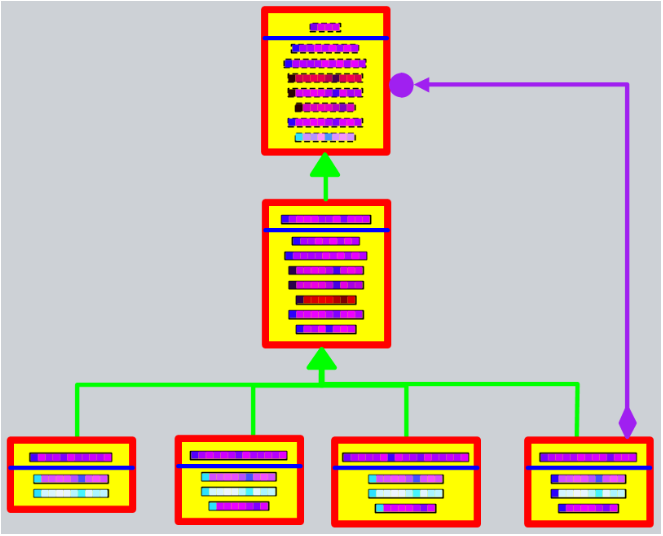
\includegraphics[scale=0.75]{figures/colored_uml.png}
    \caption{\textit{Colored UMl} für eine Mikroarchitektur}
    \label{fig:colored_uml}
\end{figure}

Die Abbildung \ref{fig:colored_uml} zeigt von Wang et al. erstelltes Exampler für \textit{Colored UML}~\cite[S. 11]{app12178718}. Wie aus der Abbildung \ref{fig:colored_uml} zu entnehmen ist, werden Bezeichner, Modifizierer und Kanten für die Assoziation farblich und/oder symbolisch enkodiert.
Hierbei ist zu erwähnen, dass die Enkodierung von Kalssenattributen im Kontext dieser Arbeit von Wang et al, nicht berücksichtigt wird.
Die Rechtecke, die in Sektion aufgeteilt, beschreiben die Klassen im Klassendiagramm. Die obere Sektion beinhaltet den Klassenbezeichner und dessen Modifzierer, während die untere Sektion die Methodenname und deren Modizierer beinhaltet. 
Jeder Bezeichner werden als Sequenzen von Charaketern aufgefasst, in diesem für jeden Charakter algorithmisch eine Farbe aus dem Rot-Grün-Blau Farbraum ermittelt wird~\cite[S. 9, S. 10]{app12178718}.
Jedem Charakter wird algortihmisch eine Farbe aus dem Rot-Grün-Blau Farbraum zugewiesen~\cite[S. 6]{app12178718}. Modifizierer für Methoden werden als Teil der Charaktersequenz betrachtet und mitenkodiert, während die Modifizierer für Klassen im Rand des Recktecks enkodiert, welches die Farben für den Klassenbezeichner umschließt~\cite[S. 6]{app12178718}.
Die Kanten des Klassendiagramms, welche die Assozation enzwischen Entitäten darstellt, werden in \textit{Colored UML} farblich annotiert und mit symbolisch an den Enden der Kanten je nach Art der Assoziation enkodiert~\cite[S. 6]{app12178718}.

Zunächst werden im ersten Schritt des Prozesses aus Quelldateien durch Software-Werkzeuge UML Klassendiagramme erstellt, welche im nächsten Schritt un \textit{Colored UML} umgewandelt.
Auf den enkodierten Quelldaten wird Bildklassifizierer VGGNet angewendet, welches Features aus der Eingabe als numerischen Vektor mit einer Länge von 1000 extrahiert. Im finalen Schritt dient dieser Feature-Vektor als Einhabe für eine Single Vector Maschine, welches die Klassenzifikation übernimmt, zu welchen Entwurfsmuster die Einagbe zugeordnet werden kann~\cite[S. 13]{app12178718}.
Das hier presentierte Modell für zwölf Design Patterns traniert~\cite[S. 15]{app12178718}
Für das Training des Models und Evaluierng der Resulate des Verfahrens wurden drei Open Source Software-Systeme verwendet. Zusätzlich wird das Verfahren auf mit drei nicht Maschine Learning Verfahren auf \textit{Precision} und \textit{Recall} verglichen~\cite[S. 20]{app12178718}.
Nach eigener Evaluering von Wang et. al weist das ihrerseits entwickelte Verfahren verglichen zu den anderen Methoden ähnliche oder bessere Klassifizierungsleistung auf~\cite[S. 22]{app12178718}.

\pagebreak

Ein weitere Möglichkeit, um Entwurfsmuster im Quellcode zu ermittelt, ist die Extraktion von Metriken und Maßen aus dem Quellcode, welche typische Instanzen für das betrachtete Design Pattern beschreiben.
In ihrer Arbeit fokussieren sich Uchiyama auf diesen Punkt und definieren einen Katalog aus Metriken und Maßen, die als Eingabe für einen Klassifizierer verwendet wird.
In dieser Arbeit definieren Uchiyama et al. Design Patterns als eine Summe von Strukturen von Klassen, Schnittstellen und Objekten, die im Kontext des Entwurfsmuster einer Rolle zugeordnet werden, und ihren Relationen zueinander.~\cite[S. 3]{Uchiyama2014}.
Im Kontext dieser Arbeit limitieren sich Uchiyama et al. auf die Erkennung fünf Entwurfsmuster mit insgesamt 12 Rollen im Quellcode.~\cite[S. 4]{Uchiyama2014}.
Für dieses Rollen werden Metriken und Maße ermittelt, die charakteritisch die Rollen beschreiben.
Um die Elemente des Katalogs zu bestimmen, wird in dieser Arbeit die Goal-Question-Metric Methode angewendet~\cite[S. 4]{Uchiyama2014}.
Hierbei werden gezielt Fragen, mit dem Ziel, die jeweilige Rolle zu bestimmen. Für die Beantwortung dieser Fragen werden Metriken bzw. Maße definiert, und als Teil des Katalogs aufgenommen.
Um die zwölf Rollen zu bestimmen, definieren Uchiyama et. al folgende Metriken~\cite[S. 7]{Uchiyama2014}:


\begin{table}[H]
    \centering
    \begin{tabular}{|c|c|}
        \hline
        Abkürzung & Beschreibung\\
        \hline
        NOF & Anzahl der Felder\\
        NSF & Anzahl der statischen Felder\\
        NOM & Anzahl der Methoden\\
        NSM & Anzahl der statischen Methoden\\
        NOI & Anzahl der implemtierten Schnittstellen\\
        NOAM & Anzahl abstrakter Methoden\\
        NORM & Anzahl der überschriebenen Methoden\\
        NOPC & Anzahl der privaten Konstruktoren in der Klasse\\
        NOTC & Anzahl der Konstruktoren mit Objektparametern\\
        NOOF & Anzahl der an Feldern mit Objekttypen\\
        NCOF & Anzahl der anderer, die die Klasse/Schnittstelle als Feld referenzieren\\
        NMGI & Anzahl der Methoden, die Instanzen generieren\\
        \hline 
    \end{tabular}
    \caption{Metriken und Maße für Rollen nach Uchiyama et al.}
    \label{table:metrics}
\end{table}

Im ersten Schritt ihrer Methode extrahieren Uchiyama et al. die aus der Tabelle~\ref{table:metrics} definierten Metriken für jede Entität aus den Quelldateien. 
Dieser Metriken werden als Vektor aufgefasst und diesen als Eingabe für eine Klassifizierer verwendet, welche die Rollenzuweisung für den Eingabevektor bestimmt~\cite[S. 5]{Uchiyama2014}.
Bei dem in dieser Methodik angewandten Klasszfizierer handelt es sich um ein neuronales Netzwerk~\cite[S. 4]{Uchiyama2014}.
Die Ausgabe des Klassifizieres sind Werte, mit welcher Sicherheit der Eingabevektor zu der jeweiligen Rolle zugeordnet werden kann~\cite[S. 5]{Uchiyama2014}.
Anhad dieser Ausgabe werden die Rollen mit dem höchsten Konfidenzwert pro Eingabevektor als Eingabe für die Bestimmung des Entwurfsmusters genommen. Unter der Berücksichtigung der Relationen der Rollen in dem potenziellen Entwurfsmuster wird ein Wert ermittelt,
welcher angibt, mit welcher Wahrscheinlichkeit die Rollen zu dem jeweiligen Design Pattern passen.~\cite[S. 6]{Uchiyama2014}. Je höher dieser Wert, desto höher die Konfidenz, dass es sich hierbei um das Entwurfsmuter handelt.
Für das Training ihrers Klasszfizierers nutzen Uchiyama et al. 60 Instanzen aus klein-skalierten Software-Systemen und 158 aus drei größeren Open Source Software-Systemen.~\cite[S. 7]{Uchiyama2014}
Für die Evaluierung der Methode bedienen sich Uchiyama et. al den Metriken der \textit{Precision} und \textit{Recall} und ermitteln diese für Design Pattern.
Dabei werden für Instanzen aus klein-skalierten Software-System besserre \textit{Precison}- und \textit{Recall}-Werte verglichen zu den Instanzen aus den Open Source Software-Systemen~\cite[S. 8]{Uchiyama2014}

\smallbreak

Durch Charakterisierung der Klassen, Schnittstellen und Objekte durch Metriken und Maße sind zwar der Rückschlüsse auf Struktur und Verhalten möglich, jedoch wird der lexigraphische und syntaktische Aspekts nicht mit berücksichtigt.
Um den gegegen zu wirken, präsentieren Nazar et. al in ihrer Arbeit ihre Methode namens DPD\textsubscript{F}, die diese Aspkete des Quellcodes mitberücksichtigt~\cite[S. 1]{Nazar2020}.
Initial wird aus dem Quellcode durch stattische Codeanalyse folgende Metriken extrahiert~\cite[S. 5]{Nazar2020}:

\begin{table}[H]
    \begin{tabular}{|c|c|}
        \hline
        Featurebezeichner & Beschreibung\\
        \hline
        ClassName & Name der Java Klasse\\
        ClassModifiers & Public, Protected und Private-Schlüsselwörter\\
        ClassImplements & Binäres Features (0/1), falls eine Schnittstelle implementiert wird\\ 
        ClassExtends & Binäres Features (0/1), ob Klasse von einer anderen vererbt\\
        MethodName & Methodname in der Klasse\\
        MethodReturnType & Typ des Rückgabewerts einer Methode\\
        MethodBodyLineType & Art des Ausdrucks (z.B Variablenzuweisung, Boolean-Ausdruck)\\
        MethodNumVariables & Anzahl der Variablen/Attribute in der Klasse\\
        MethodNumMethods & Anzahl der Methodenaufrufe in der Klasse\\
        MethodsNumLine & Anzahl der Zeilen in Methode\\
        MethodIncomingMethod & Anzahl an Methoden, die in eine Methode aufruft\\
        MethodIncomingName & Name der Methoden, die von der Methode aufgreufen werden\\
        MethodOutgoingMethod & Anzahl ausgehender Methoden\\
        MethodOutgoingName & Name der ausgehenenden Methoden\\
        \hline  
    \end{tabular}
    \caption{Extrahierte Features für DPD\textsubscript{F}}
    \label{table:dpdf_features}
\end{table}

Die ersten vier in der Tabelle \ref{table:dpdf_features} aufgelisteten Features werden pro Klasse, während die restlichen elf pro Methode in der Klasse ermittelt werden.
Jeder ist dieser Features wird als eine Auflistung von Schlüssel-Werte-Paaren in natürlicher Sprache abgelegt.
Da jede Auflistung der Evaluierung einnes Methodenblocks entspricht, werden Features von der Klasse, in der die Methode implementiert ist, in diesen wiederholt.
Jede Auflistung wird als Zeile in natürlicher Sprache in einer Textdatei zusammengefasst. Das dabei entstehende Format wirtd von Nazar at al. als Syntactic and Lexical Representation (SSLR) benannt~\cite[S. 1]{Nazar2020}.
Um SSLR in eine numerische Form zu bringen, wird SSLR als Eingabe für Word2Vec verwendet, welches für jeden Token mit Einbezug der umgebenden Tokens als Kontext der SSLR einen numerischen Vektor mit einer Länge von 100 determiniert, dass das jeweilige Token repräsentiert~\cite[S. 6]{Nazar2020}.
Die resultierenden Vektoren dienen als Eingabe für einen Random Forest Classifier, welches das meist passende Entwurfsmuster bestimmt~\cite[S. 7]{Nazar2020}
Für das Training der Modelle und Evaluierung von DPD\textsubscript{F} wird ein eigener Korpus angelegt, bestehend aus Quelldateien aus \textit{Github Java Corpus}. Durch Crowd-Sourcing wurden zwölf Entwurfsmuster mit je 100 Instanzen identifiziert~\cite[S. 4]{Nazar2020}.
Für die Evaluierung wird für jedes betrachtete Design Pattern im Korpus der \textit{F1}-, \textit{Precision}- und \textit{Recall}-Wert ermittelt. Nach eigener Evaluierung von Nazar et al. mit dem selbsterstellten Korpus, erreicht ihre Methode im Durchschnitt einen \textit{Precision}-Wert von über 80\% und einem \textit{Recall}-Wert von 79\%~\cite[S. 8]{Nazar2020}.   

%%TODO: Start with this Research on Design Pattern Detection Method Based on UML Model with Extended Image Information and Deep Learning


\subsection{Similarity-Scoring Ansätze}

\subsection{Diverse Ansätze}



